%!TEX root = ../dokumentation.tex

\chapter{Umsetzung}\label{cha:Umsetzung}
<Allgemeine Beschreibung des Inhalts des Kapitels.>

\section{Verarbeitungsprozess}
<Hier sollte der Prozess der Anwendung geplant werden. wo liegen die Daten? wie findet der zugriff statt? nach welchem schema sind sie abgelegt und benannt? Außerdem sollte klar werden wie die Informationen verarbeitet werden. ein großer map reduce oder eine verkettung mehrerer mapper und reducer? Außerdem muss das ausgabeformat festgelegt werden. Bzw. zwei alternativen. eine für wenn die anwendung performant genug ist um als check skript zu laufen, und eine für den fall das nicht.>

\begin{figure}
	\centering
	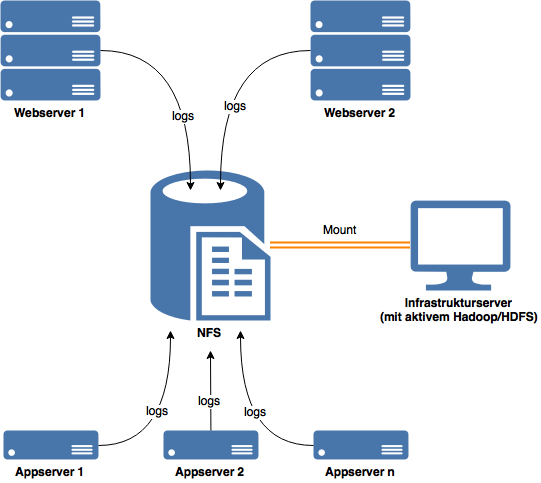
\includegraphics[width=.8\textwidth]{Infrastruktur.png}
	\caption{DUMMY: Aufbau der Infrastruktur}
	\label{fig:AufbauInfrastruktur}
\end{figure}

\section{Implementierung von Properties}
<Beschreibung wie Properties programmiert werden. Wie werden diese in der Anwendung umgesetzt? Welche Rolle spielen Properties für den generischen Teil der Anwendung?>

\section{Grundlagen für Datenverarbeitung}
<Beschreibung der Entwicklung für die Grundlagen zur Datenverarbeitung. Welche Klassen werden dabei verwendet? Welches System liegt dahinter? Warum dieses System? Dabei nicht nur auf die Speicherung von Daten eingehen sondern auch auf das Lesen von Dateien.>

\section{Bestimmung des Aufbaus der Logfiles}
<Wie sehen die Logfiles aus? Welche Formate haben sie? Welche rolle spielen diese bei der Datenverarbeitung? Welche Informationen sind die richtigen Informationen?>

\section{Implementierung von MapReduce}
<Beschreibung vom Kern der Anwendung. Wie wird der Algorithmus umgesetzt? Welche Klassen/Methoden sind notwendig? Wie unterscheidet sich die Implementierung bei unterschiedlichem Input. Spielt das überhaupt eine Rolle oder muss es nur Text sein? Welches Ergebnis bekommt man und in welcher Form?>